% Its PDF copy is retained locally; generated PDFs are not committed.
\documentclass[11pt,a4paper]{article}

\usepackage[margin=25mm]{geometry}
\usepackage[T1]{fontenc}
\usepackage[utf8]{inputenc}
\usepackage{lmodern}
\usepackage{amsmath}
\usepackage{booktabs}
\usepackage{graphicx}
\usepackage{tabularx}
\usepackage{array}
\usepackage{caption}
\usepackage{hyperref}
\usepackage{tikz}
\usepackage{pdflscape}
\usepackage{placeins}
\usetikzlibrary{positioning,fit,arrows.meta}

\newcommand{\projecttitle}{Singapore Rainfall Analysis and Prediction}

\hypersetup{
  pdftitle={\projecttitle},
  pdfauthor={DAM MINH TIEN; Nguyen Minh Duc; Vu Nhat Nguyen Thu},
  pdfsubject={DSA5208 Project 2 final report},
  colorlinks=true,
  linkcolor=black,
  citecolor=black,
  urlcolor=blue
}
\setlength{\parskip}{0.45em}
\setlength{\parindent}{0pt}
\captionsetup{font=small,labelfont=bf}

\newcommand{\figpath}{figures/full-20261012}

\begin{document}

\hypersetup{pageanchor=false}
\begin{titlepage}
  \centering
  \vspace*{35mm}
  {\Large DSA5208 Project 2\par}
  \vspace{10mm}
  {\LARGE\bfseries \projecttitle\par}
  \vfill
  {\large DAM MINH TIEN\par}
  {\normalsize Student ID: A03355091E\par}
  \vspace{4mm}
  {\large Nguyen Minh Duc\par}
  {\normalsize Student ID: A0308841A\par}
  {\normalsize E1404392@u.nus.edu\par}
  \vspace{4mm}
  {\large Vu Nhat Nguyen Thu\par}
  {\normalsize Student ID: A0306148H\par}
  {\normalsize E1376354@u.nus.edu\par}
  \vspace{10mm}
  {\large 17 October 2026\par}
\end{titlepage}

\hypersetup{pageanchor=true}
\pagenumbering{roman}
\section*{Abstract}
This report analyses NEA five-minute rainfall records from 2017 to 2024. Wet-
reading frequency ranged from 1.94\% to 3.20\%. Because no station met the
90\% annual-coverage rule in every year, annual comparisons use a changing
station network. For Task 2, five candidates were compared on a 10\% sample
of 2022 after hyperparameter validation on 2021. The selected GBT-B model was
refitted on 2017--2022 data and calibrated on 2023. PAVA was then applied to
enforce non-increasing exceedance probability as the rainfall threshold
increased. On the 2024 evaluation period, final PAVA GBT-B achieved PR-AUC
0.6345 and Brier score 0.01958 at 0.5~mm, compared with 0.0732 and 0.03436
for the climatology baseline. PAVA removed all monotonicity violations across
31.87 million adjacent threshold pairs.

\begingroup
\small
\setlength{\parskip}{0pt}
\tableofcontents
\endgroup
\clearpage
\pagenumbering{arabic}

\section{Introduction}
The report uses the National Environment Agency's Historical Rainfall across
Singapore collection, timestamped in Singapore Time. The catalog warns that
records may be missing and have not undergone climate-record quality control~\cite{nea}.

Task 1 describes all eight years. For Task 2, 2017--2020 supports hyperparameter
training, 2021 supports hyperparameter validation, 2022 is used for candidate
selection, the selected model is refitted on all valid 2017--2022 windows, 2023
is used for probability calibration, and 2024 is reserved for final evaluation.

\section{Data and cleaning}
\subsection{Input and timestamp handling}
The eight annual source files contain 48,538,713 rows and 12 columns. The
rainfall field
is NEA reading type \texttt{TB1 Rainfall 5 Minute Total F}, in millimetres. The
download time was not recorded. The project's
interval-end convention treats a reading at time $t$ as rainfall accumulated
over $(t-5\text{ min},t]$; this is an analysis assumption, not an NEA-confirmed
timestamp definition.

Early 2017 records systematically end at second 59; later 2017 and 2018--2024
records end at second 00. The same \texttt{:59} convention appears in the
official 2016 dataset, which was not used here~\cite{nea}. In 2017, 3,480,779
timestamps fell on five-minute boundaries and 1,775,327 fell one second before
them. We shifted the systematic \texttt{:59} timestamps forward by one second
to align them with five-minute boundaries and retained the source timestamps
for audit. NEA does not document the reason for this convention change. Other
off-grid timestamps were rejected.

Validation covered parsing, station IDs, timestamps, nonnegative rainfall,
date/year, reading type and unit. Duplicate station-time keys were resolved
deterministically. Coordinates were used only for the supplementary spatial
summary. Missing readings remain gaps and were not filled with zero.

\begin{table}[htbp]
\centering\small
\caption{Rainfall records retained by source year, with exclusions separated
into validation filters and duplicate resolution. The station column counts
distinct retained station IDs within that year.}
\label{tab:cleaning}
\begin{tabular}{r r r r r r}
\toprule
Year & Raw rows & Retained rows & \shortstack{Validation\\filtered} & \shortstack{Duplicate\\rows} & Stations \\
\midrule
2017 & 5,256,106 & 5,256,020 & 0 & 86 & 62 \\
2018 & 4,594,246 & 4,594,246 & 0 & 0 & 56 \\
2019 & 5,026,862 & 5,026,862 & 0 & 0 & 54 \\
2020 & 6,334,473 & 6,334,473 & 0 & 0 & 80 \\
2021 & 7,044,646 & 7,044,646 & 0 & 0 & 76 \\
2022 & 7,133,230 & 7,133,230 & 0 & 0 & 72 \\
2023 & 6,742,890 & 6,742,890 & 0 & 0 & 74 \\
2024 & 6,406,260 & 6,406,260 & 0 & 0 & 70 \\
\midrule
Total & 48,538,713 & 48,538,627 & 0 & 86 & --- \\
\bottomrule
\end{tabular}
\end{table}

The row-level audit of the 2017 source file found no records rejected by
validation. All 86 exclusions came from duplicate resolution: they shared an
existing station-time key and the same rainfall measurement. No conflicting
station-time key was excluded. The retained and excluded totals reconcile to
the raw count (Table~\ref{tab:cleaning}).

\subsection{Coverage definitions}
Coverage is the count of retained five-minute readings divided by the expected
slots (288 per calendar day) in the full calendar period, including periods
with no records. Rainfall
occurrence is the share of retained readings greater than zero; missing
readings are excluded from this denominator and are not treated as dry.
Conditional wet intensity is the mean five-minute rainfall total among
positive readings. A
station-month rainfall total is the sum of observed readings and is not
adjusted for missing slots.

Monthly summaries include station-months with at least 95\% coverage and give
each eligible station-month equal weight. For hourly summaries, the same
monthly rule applies, and each station-month-hour must also have at least 95\%
of its expected readings (12 per day for that hour). At a given hour, eligible
station-month-hour summaries receive equal weight. Because station coverage
changes across years, these summaries are not estimates for a fixed station
network.

A complete day has exactly 288 retained five-minute readings. Supplementary
complete-day estimates first average complete daily totals within each
station-month, then give each contributing station-month equal weight. The
complete-day fraction uses all expected station-days for the station IDs seen
anywhere in 2017--2024 as its denominator, so it reflects both recording
completeness and changes in station availability.

\subsection{Computing Environment and Distributed Execution}
The project ran on Google Cloud Dataproc in \texttt{asia-southeast1}. Spark
handled station-time cleaning and aggregation, rainfall-history and target
construction, threshold expansion, and MLlib model fitting and scoring across
worker executors. Table~\ref{tab:cluster} summarizes the final model cluster;
the project demonstrates distributed execution but does not evaluate
scalability.

\begin{table}[htbp]
\centering\small
\caption{Computing environment for the final GBT-B fit.}
\label{tab:cluster}
\begin{tabularx}{\linewidth}{l X}
\toprule
Platform and region & Google Cloud Dataproc, \texttt{asia-southeast1} \\
Dataproc image & \texttt{2.2.87-debian12} \\
Spark / Python & Spark 3.5.3 / Python 3.11~\cite{spark,dataprocimage} \\
Master & One \texttt{e2-standard-4}: 4 vCPU, 16~GB RAM~\cite{gceE2} \\
Workers & Eight \texttt{e2-highmem-2}: 2 vCPU and 16~GB RAM each~\cite{gceE2} \\
Executors & Eight executors, two cores each; dynamic allocation disabled \\
Worker disks & 40~GB standard persistent disk per worker \\
Storage & Google Cloud Storage for features, models and outputs \\
Interface & Dataproc Jupyter Notebook; sequential Spark job submission \\
\bottomrule
\end{tabularx}
\end{table}

\begin{table}[htbp]
\centering\footnotesize
\caption{Recorded execution for the final model and 2024 evaluation applications.}
\label{tab:job-evidence}
\begin{tabularx}{\linewidth}{p{28mm} X r}
\toprule
Workload & Recorded execution evidence & Runtime \\
\midrule
Final GBT-B fit & 207,248,820 threshold-expanded training examples. Eight worker executors (16 cores); 241 jobs, 404 stages and 25,431 tasks. Stage 21 processed 2.4~GiB with 66 tasks and wrote 52.8~MiB of shuffle data. & 12,286.9~s \\
2024 evaluation & 6,374,476 base windows (38,246,856 threshold rows). Eight worker executors (16 cores); 325 jobs, 386 completed stage attempts and 25,305 tasks. Application totals: 36.5~GiB input, 4.4~GiB shuffle read and 4.2~GiB shuffle write; saved predictions were evaluated. & 478~s \\
\bottomrule
\end{tabularx}
\end{table}

\begin{figure}[htbp]
\centering
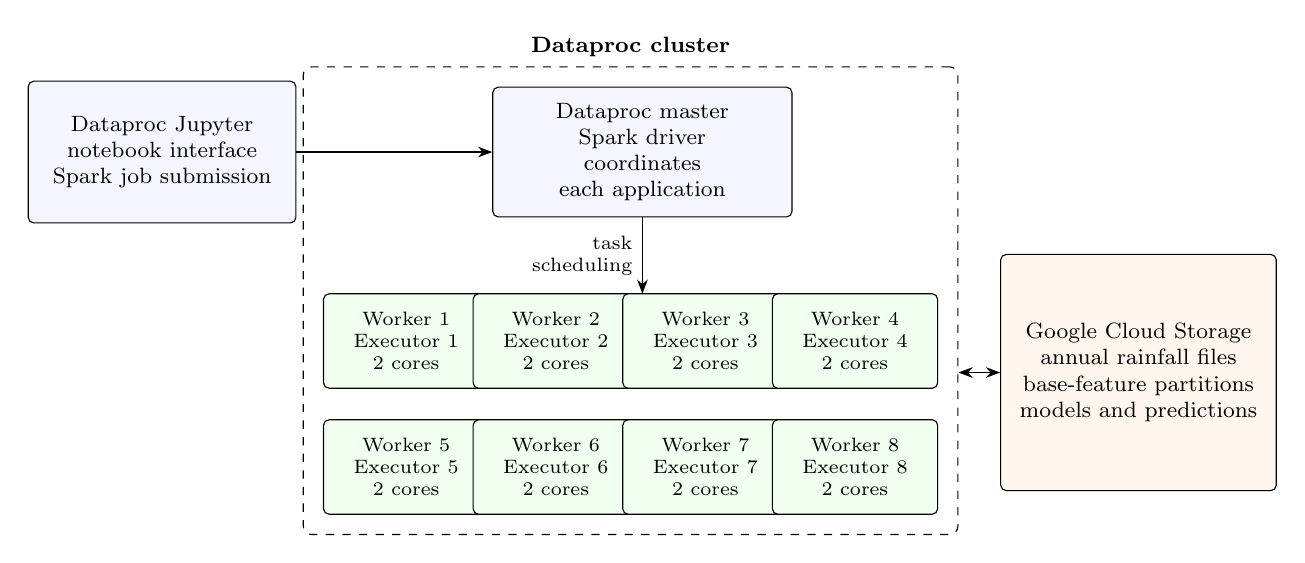
\begin{tikzpicture}[x=1mm,y=1mm,
  font=\footnotesize,
  component/.style={draw, rounded corners=2pt, align=center, inner sep=2mm,
                    fill=blue!4},
  worker/.style={component, text width=17mm, minimum height=12mm,
                 font=\scriptsize, fill=green!6},
  flow/.style={-{Stealth[length=1.8mm]}, semithick},
  dataflow/.style={{Stealth[length=1.8mm]}-{Stealth[length=1.8mm]}, semithick},
  cluster/.style={draw, dashed, rounded corners=3pt, inner sep=2.5mm,
                  fill=none}
]
  \node[component, text width=30mm, minimum height=18mm] (notebook) at (9,4)
    {Dataproc Jupyter\\notebook interface\\Spark job submission};
  \node[component, text width=34mm, minimum height=16mm] (master) at (70,4)
    {Dataproc master\\Spark driver\\coordinates each application};

  \node[worker] (w1) at (40,-20) {Worker 1\\Executor 1\\2 cores};
  \node[worker] (w2) at (59,-20) {Worker 2\\Executor 2\\2 cores};
  \node[worker] (w3) at (78,-20) {Worker 3\\Executor 3\\2 cores};
  \node[worker] (w4) at (97,-20) {Worker 4\\Executor 4\\2 cores};
  \node[worker] (w5) at (40,-36) {Worker 5\\Executor 5\\2 cores};
  \node[worker] (w6) at (59,-36) {Worker 6\\Executor 6\\2 cores};
  \node[worker] (w7) at (78,-36) {Worker 7\\Executor 7\\2 cores};
  \node[worker] (w8) at (97,-36) {Worker 8\\Executor 8\\2 cores};

  \node[cluster, fit=(master)(w1)(w2)(w3)(w4)(w5)(w6)(w7)(w8),
        label={[font=\footnotesize\bfseries]above:Dataproc cluster}] (clusterbox) {};
  \node[component, text width=31mm, minimum height=30mm, fill=orange!7] (gcs)
    at (133,-24) {Google Cloud Storage\\annual rainfall files\\base-feature partitions\\models and predictions};

  \draw[flow] (notebook.east) -- (master.west);
  \draw[flow] (master.south) -- node[left, font=\scriptsize, align=right]
    {task\\scheduling} (70,-14);
  \draw[dataflow] (clusterbox.east |- gcs.west) -- (gcs.west);
\end{tikzpicture}
\caption{Spark applications are submitted from the Dataproc Jupyter interface
to the master driver. The driver schedules work across eight two-core worker
executors, which read project data from and write results to Google Cloud
Storage.}
\label{fig:runtime}
\end{figure}

